\chapter{Results}

This chapter reports the empirical findings from two controlled experiments: a version-level ablation study across three progressively enhanced framework variants, and a cross-model comparison across three frontier language models. All quantitative results are obtained using the evaluation infrastructure described in Chapter~4.

\section{Evaluation Methodology}

\subsection{Benchmark Scenarios}

The evaluation framework defines a set of benchmark scenarios drawn from the official AWS Architecture Blog and AWS Solutions Library. Each scenario specifies a problem statement and reference architecture sourced from the official documentation.

\subsection{Natural Language Processing Metrics}

Two natural language processing (NLP) similarity metrics are employed:

\begin{itemize}
\item \textbf{METEOR} \cite{banerjee2005meteor} --- enhances lexical alignment through the incorporation of stemming and synonym matching, capturing partial semantic equivalence beyond exact token overlap.
\item \textbf{BERTScore F1} \cite{zhang2019bertscore} — computes cosine similarity between contextual embeddings derived from BERT for candidate and reference texts, providing a model-based estimate of semantic similarity.
\end{itemize}

Both metrics are computed against the human-authored reference architecture text supplied with each scenario. Three independent runs per configuration are executed to estimate result stability.
\subsection{LLM-as-a-Judge}

The evaluation also includes the \textbf{LLM-as-a-Judge} paradigm \cite{zheng2024judging}, in which an independent frontier model scores each generated architecture across the six structured dimensions defined in Section~\ref{subsec:judge_rubric} of Chapter~4 (completeness, technical accuracy, security, scalability, best practices alignment, and specificity) on an integer scale of 1 to 10. The composite judge score is the arithmetic mean of these six dimension scores. The judge model used throughout this work is \texttt{claude-sonnet-4-6}.



\subsection{Experiment Design}

Two controlled experiments are conducted:

\begin{itemize}
    \item \textbf{Experiment 1 — Version Ablation}: Three framework variants are compared across all models (GPT-5.4, Claude Sonnet 4.6, Gemini 3.1 Pro). This isolates the contribution of ground truth validation, multi-agent decomposition and the Evaluator-Optimizer loop, respectively.
    \item \textbf{Experiment 2 — Model Comparison}: Three frontier models (GPT-5.4, Claude Sonnet 4.6, Gemini 3.1 Pro) are compared using the full Evaluator-Optimizer framework as the fixed variant.
\end{itemize}


\section{Experiment 1: Framework Version Ablation}
\label{sec:exp1}

The first experiment compares the three progressively enhanced framework variants defined in Section~\ref{subsec:runner_variants} of Chapter~4 (Baseline Single Prompt LLM, Agentic Framework, and Complete Evaluator-Optimizer Loop Framework) across all three models: GPT-5.4, Claude Sonnet 4.6, and Gemini 3.1 Pro.

\begin{table}[htbp]
\centering
\caption{Version Comparison — Average Across All Models (GPT-5.4, Claude Sonnet 4.6, Gemini 3.1 Pro)}
\label{tab:table_version_summary}
\begin{tabular}{lccc}
\toprule
Version & METEOR & BERTScore F1 & Judge Total \\
\midrule
Baseline - Single Prompt LLM & 0.254 & 0.811 & 9.028 \\
Agentic Framework & 0.265 & 0.806 & 9.112 \\
Evaluator Optimiser Loop Framework & 0.251 & 0.809 & 9.166 \\
\bottomrule
\end{tabular}
\end{table}

 Table~\ref{tab:table_version_summary} presents the aggregate METEOR, BERTScore F1, and judge total scores for each framework variant on the benchmark scenarios. 

The judge total increases across variants: from 9.028 for the single-prompt baseline, to 9.112 for the agentic framework, and further to 9.166 for the full Evaluator-Optimizer loop. This stepwise progression demonstrates that both the multi-agent decomposition stage and the iterative validation stage contribute independently to architectural quality uplift, with the largest individual increment attributable to the introduction of domain-specialised parallel generation.

Across the six evaluation dimensions—completeness, accuracy, security, scalability, best practices, and specificity—scores increase across variants, with the most notable improvements observed in accuracy, which contributes most to the overall performance gains. Figure~\ref{fig:chart_combined_heatmap} visualises these results.

\begin{figure}[htbp]
\centering
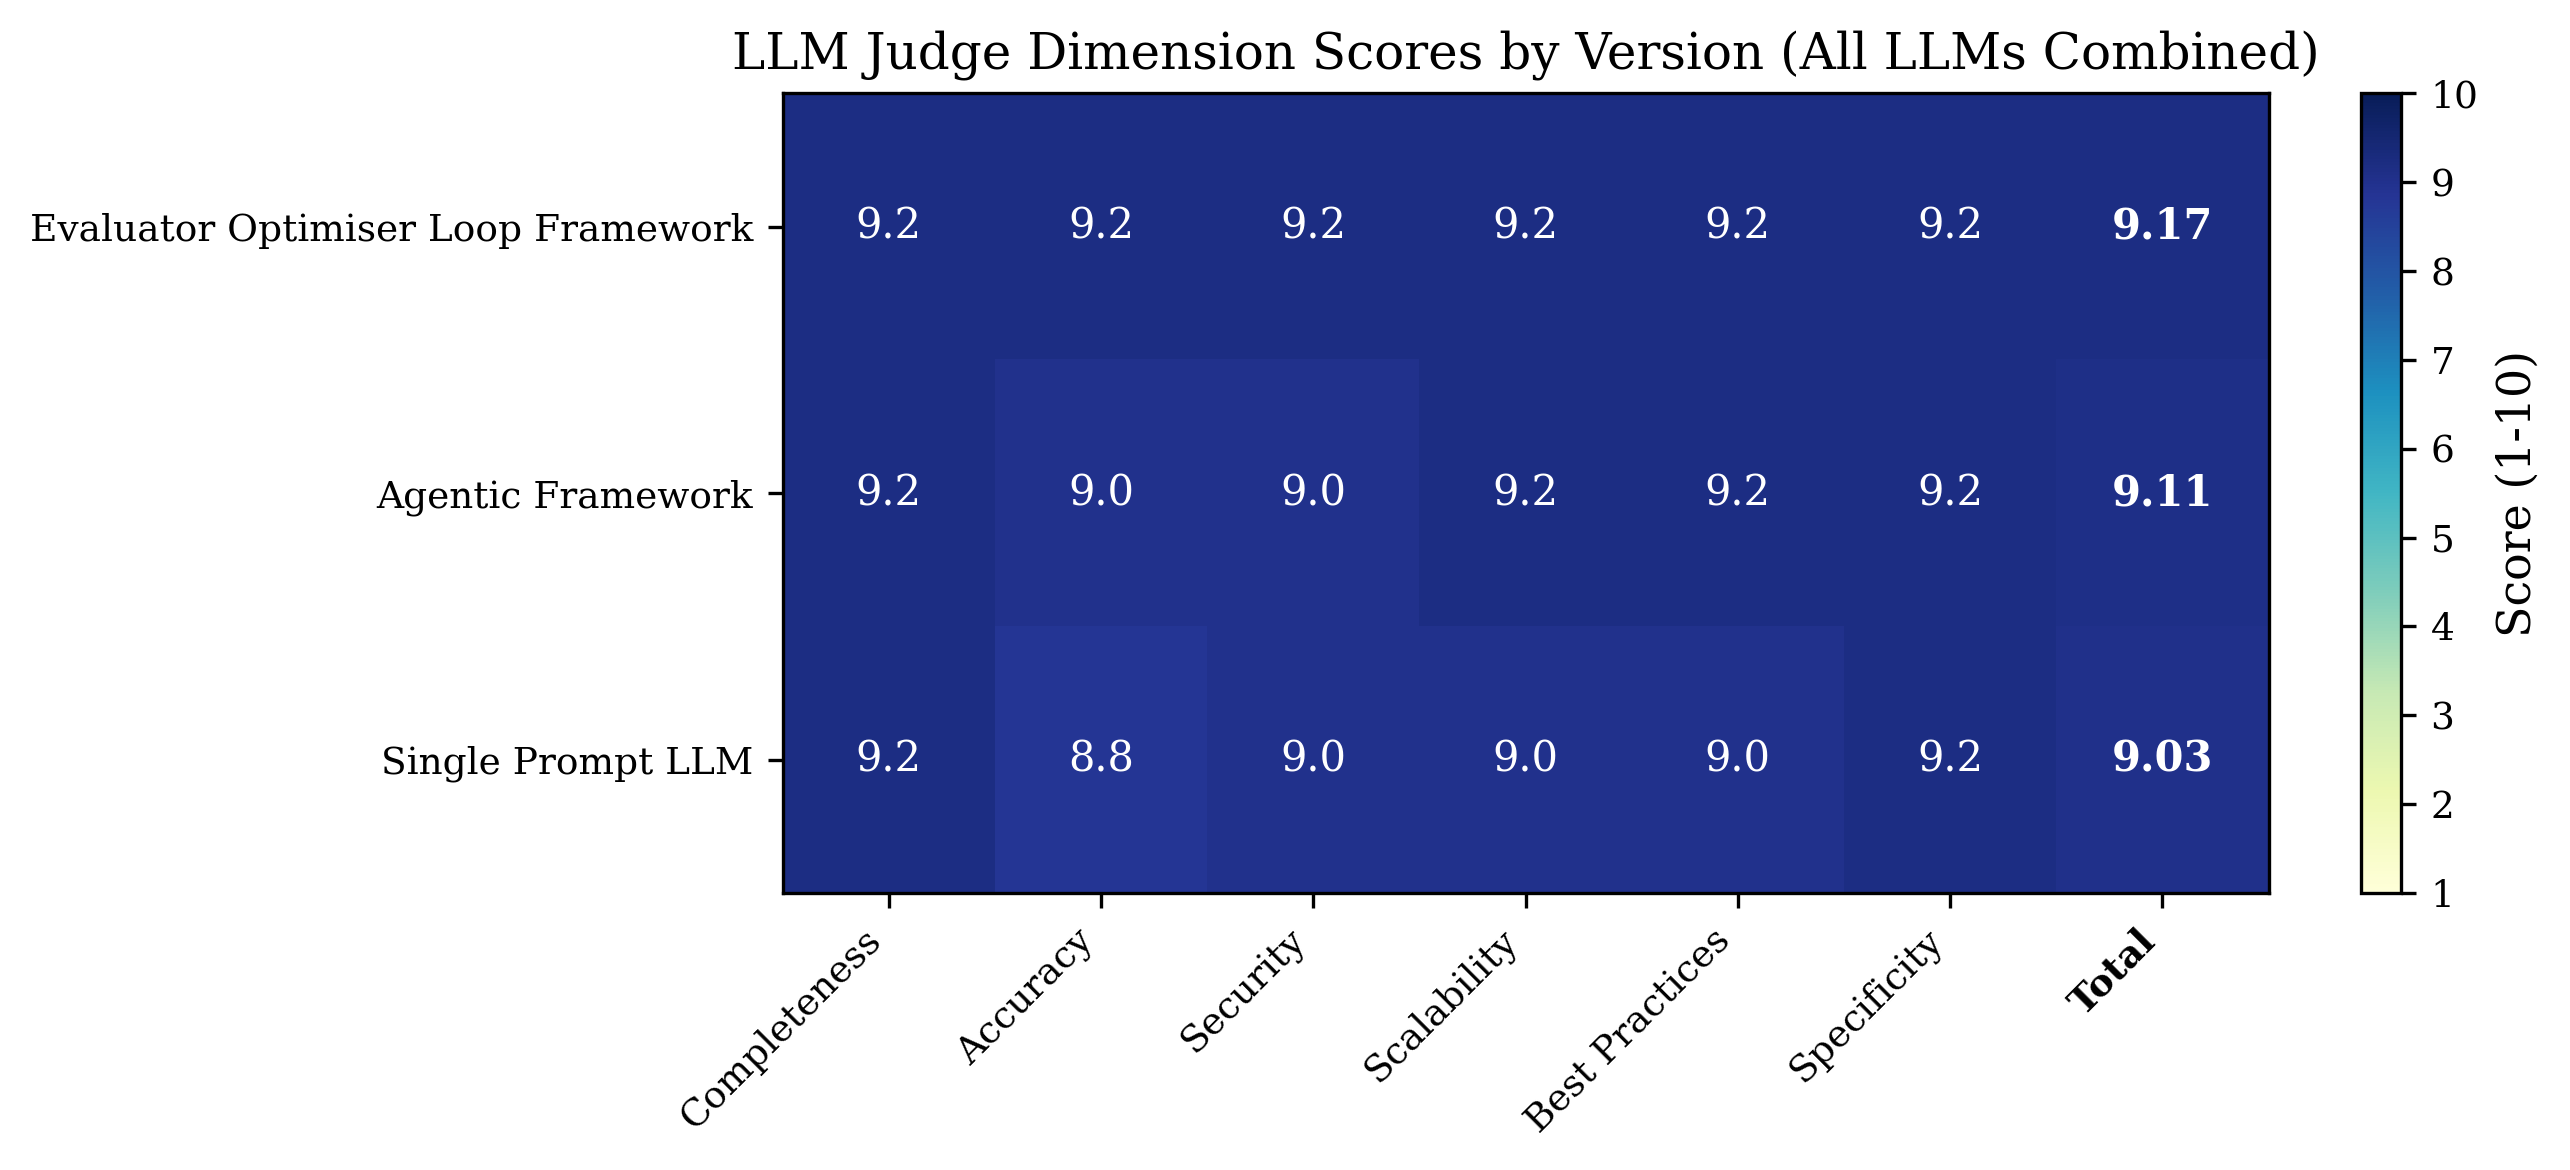
\includegraphics[width=\textwidth]{./figures/chart_combined_heatmap.png}
\caption{Aggregated distribution of LLM judge dimension scores across framework variants}
\label{fig:chart_combined_heatmap}
\end{figure}


METEOR does not, however, exhibit a monotonic relationship with architectural quality. The full framework achieves a METEOR score of 0.251, which is lower than that of the agentic variant 0.265, despite attaining the highest overall judge score. This dissociation—where METEOR decreases while judged quality increases—provides evidence that token-overlap metrics are insufficient for evaluating open-ended architecture generation tasks. This effect can be attributed to lexical divergence introduced by the RAG mechanism, which surfaces detailed technical content from official documentation that is absent from high-level reference summaries.

This METEOR variation reflects differences in surface wording rather than a decline in conceptual fidelity. Indeed, the ablation study reproduces this structural dissociation at scale: as the validation loop enforces the inclusion of specific service-level configuration details, the generated outputs become more technically precise while diverging further lexically from the reference text.

Similarly, BERTScore remains largely invariant across all three variants 0.804 to 0.811, indicating that semantic similarity to a single reference document is an insensitive measure of improvements in architectural quality.

\section{Experiment 2: Cross-Model Comparison}
\label{sec:exp2}

The second experiment holds the framework variant constant at the full Evaluator-Optimizer loop and varies the language model across three frontier systems: GPT-5.4, Claude Sonnet 4.6, and Gemini 3.1 Pro. The reasoning tier (supervisors and synthesizers) and the execution tier (domain architects and validators) both use the same model within each configuration, enabling a clean comparison of end-to-end model capability within the framework.

\begin{table}[htbp]
\centering
\caption{LLM Judge Dimension Breakdown by Model (Evaluator Optimiser Loop Framework)}
\label{tab:model_summary}
\resizebox{1.05\textwidth}{!}{
\begin{tabular}{lccccccc}
\toprule
Model & Completeness & Accuracy & Security & Scalability & Best Practices & Specificity & Total \\
\midrule
Claude Sonnet 4.6 & 9.5 & 9.0 & 9.5 & 9.5 & 9.5 & 9.5 & 9.4167 \\
GPT-5.4 & 9.0 & 9.5 & 9.0 & 9.0 & 9.0 & 9.0 & 9.083 \\
Gemini 3.1 Pro & 9.0 & 9.0 & 9.0 & 9.0 & 9.0 & 9.0 & 9.0 \\
\bottomrule
\end{tabular}
}
\end{table}

Table~\ref{tab:model_summary} presents aggregate results. Claude Sonnet 4.6 records the highest judge total at 9.415, followed by GPT-5.4 at 9.083 and Gemini 3.1 Pro at 9.0. Claude Sonnet 4.6 achieves 9.5 on Completeness, Security, Scalability, Best Practices, and Specificity, with Technical Accuracy at 9.0, yielding an aggregate of 9.415. GPT-5.4 scores 9.5 on Technical Accuracy but 9.0 across the remaining dimensions (aggregate 9.083), suggesting superior precision in service integration details but slightly lower breadth. Gemini 3.1 Pro scores a uniform 9.0 across all six dimensions, indicating consistent but undifferentiated performance without pronounced strengths in any specific pillar.

Figures~\ref{fig:model_heatmap} visualise the cross-model comparison.

\begin{figure}[htbp]
    \centering
    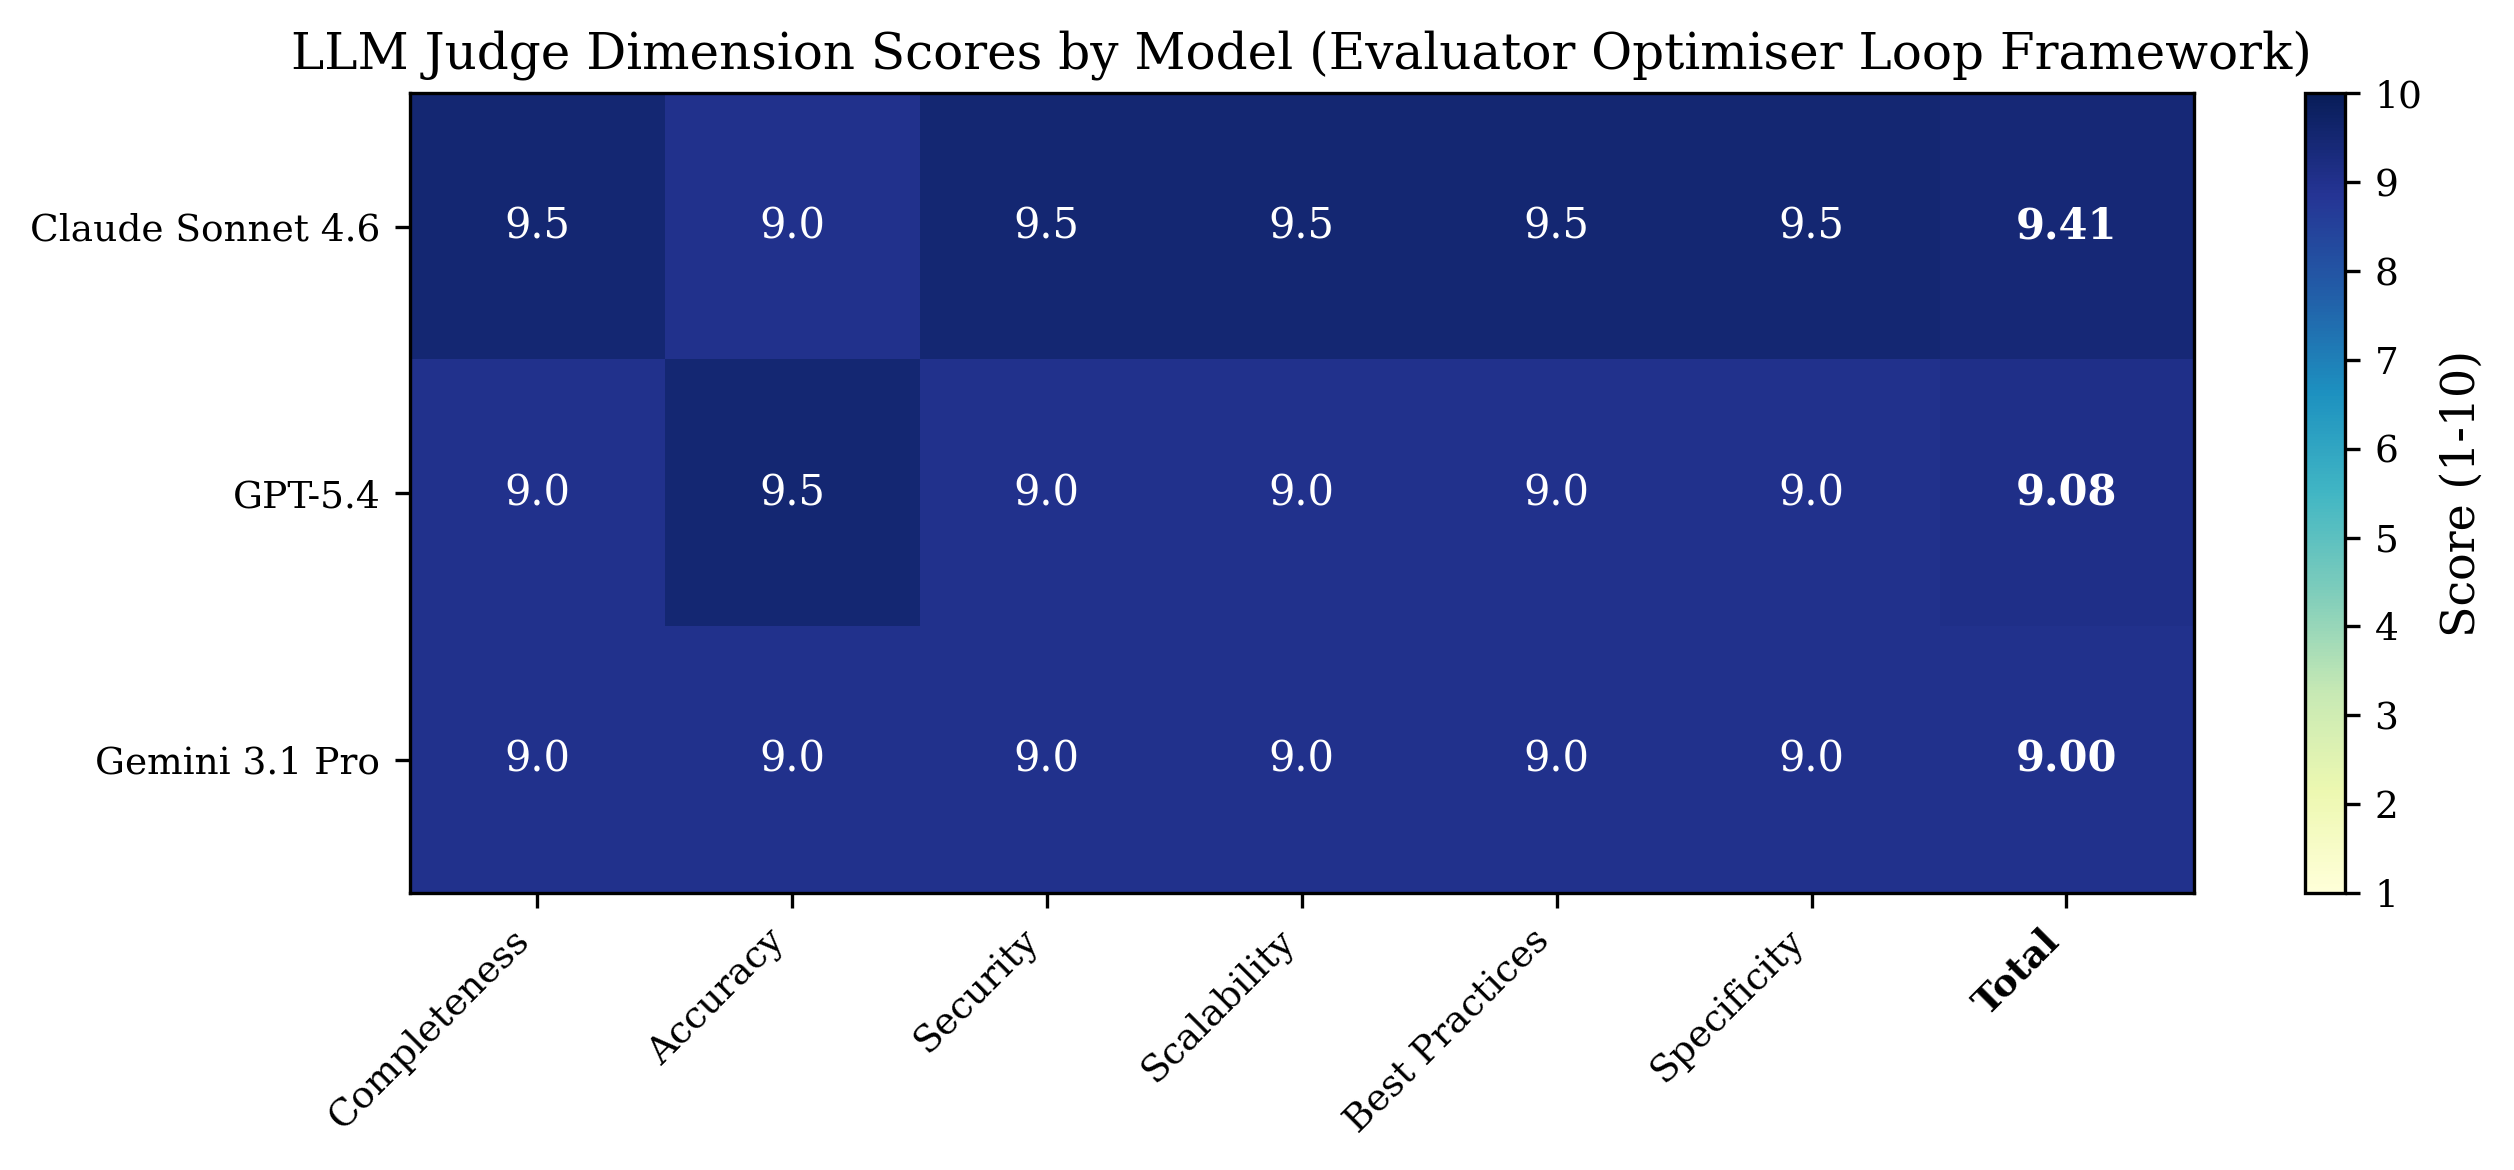
\includegraphics[width=\textwidth]{./figures/chart_model_heatmap.png}
    \caption{Heatmap chart of the six LLM judge dimensions for each model under the full framework.}
    \label{fig:model_heatmap}
\end{figure}

\section{Interpretation and Discussion}
\label{sec:discussion}
% ─────────────────────────────────────────────────────────────────────────────

\subsection{Value of the Iterative Validation Loop}

The version ablation results affirm the central design hypothesis: an Evaluator-Optimizer loop that routes generated architectures through parallel domain validators and feeds structured deficiency feedback back into the generation subgraph produces measurably higher-quality outputs than either a single-prompt baseline or a multi-agent system without validation. The results reveal that both architectural stages contribute incrementally to quality: the agentic decomposition step lifts the judge total from 9.028 (baseline) to 9.112 (+0.084), while the addition of the Evaluator-Optimizer loop raises it further to 9.166 (+0.054), for a cumulative gain of 0.138 points over the baseline. This stepwise progression indicates that multi-agent domain decomposition independently contributes to architectural quality — through parallel specialisation and tool-augmented retrieval — and that the validation loop provides a complementary, additive improvement by enforcing correctness and completeness through structured feedback propagation. While these margins are modest in absolute magnitude, the qualitative trace in Section~\ref{sec:workflow_trace} of Chapter~4 illustrates that they correspond to the progressive addition of concrete, deployment-critical configuration details that would meaningfully affect a real-world deployment. In production cloud deployments, omitting such details can constitute a security or compliance gap; the numeric gaps therefore understate the practical importance of both the multi-agent decomposition and the iterative validation mechanism. 

\subsection{NLP Metric vs.\ Expert Quality Dissociation}

First experiment shows that METEOR and BERTScore F1 exhibit weak or inverse correlation with expert judge scores. In Experiment 1, the best-judged variant (full framework) has a lower METEOR than the agentic draft. This dissociation is consistent with the ``one-to-many'' nature of cloud architecture design: a problem such as ``design a three-tier serverless web application'' admits many architecturally sound solutions that may differ substantially in vocabulary, service selection, and configuration strategy. NLP metrics that compare against a single fixed reference inherently penalise valid alternative solutions. This finding justifies the choice of LLM-as-a-Judge as the primary quality signal over token-overlap metrics.

\subsection{Judge Bias Caveat}
\label{subsec:judge_bias}

A methodological limitation warrants explicit acknowledgement. The judge model (\texttt{claude-sonnet-4-6}) belongs to the same model family as one of the three test subjects. Research on LLM-as-a-Judge pipelines has documented a self-enhancement bias, wherein a model assigns higher scores to outputs that are structurally or stylistically similar to its own generation patterns \cite{zheng2024judging}. Claude Sonnet 4.6's leading judge total should therefore be interpreted with caution: a fraction of its advantage over GPT-5.4 and Gemini 3.1 Pro may reflect evaluator-subject alignment rather than a genuine quality differential. Notably, the gap between the top two models is comparable in magnitude to Claude's standard deviation across runs further cautioning against strong interpretive claims. 

\subsection{Practical Considerations}

All three evaluated models produce architecturally sound outputs with judge scores at or above 9.0 under the full framework. This high performance floor indicates that the framework's multi-agent decomposition, two-stage RAG grounding, and iterative validation collectively provide a strong quality scaffold that is relatively robust to the choice of the underlying language model. In deployment scenarios where API cost or model availability is a constraint, GPT-5.4 offers a strong and well-tested default. Gemini 3.1 Pro, despite its lower judge score, produces outputs with the highest surface similarity to official reference architectures, which may be advantageous in contexts where alignment with documented patterns is prioritised over configuration specificity.

\subsection{Scope and Generalisability}

The evaluation presented in this chapter is limited to a set of benchmark scenarios representing relatively well-defined architectural patterns, for which reference solutions are comprehensive and service coverage is clearly specified. As these patterns may overlap with knowledge already captured during the training of frontier language models, even single-shot LLM approaches are likely to produce strong baseline results. However, this framework is likely to show greater advantages on more novel or less well-defined problem settings, where structured decomposition, retrieval grounding, and iterative validation become increasingly important for ensuring architectural correctness and completeness.

% ─────────────────────────────────────────────────────────────────────────────
\section{Summary}
% ─────────────────────────────────────────────────────────────────────────────

This chapter presented two controlled experiments evaluating the framework. Experiment 1 established that both architectural stages contribute incrementally to output quality, demonstrating that multi-agent domain decomposition and iterative validation each provide independent, additive quality improvements. Experiment 2 demonstrated that all three evaluated frontier models — GPT-5.4, Claude Sonnet 4.6, and Gemini 3.1 Pro — perform at a high level within the framework, achieving high judge scores. Claude Sonnet 4.6 records the highest composite judge score, though this result is subject to the self-evaluation bias caveat associated with the choice of judge model. A consistent inverse relationship between surface-level NLP metrics and expert judge scores in experiments validates the methodological choice to adopt LLM-as-a-Judge as the primary evaluation paradigm for open-ended cloud architecture generation tasks. These results show that the framework functions as a model-agnostic platform for automated cloud architecture generation and validation, with the iterative feedback loop as the primary quality-differentiating mechanism.

